\chapter{Group organisation dossier} \label{groupdossier}

\section{Internal Rules}

\subsection{Scope}
The purpose of this document is to provide a comprehensive overview of the internship experience by documenting and showcasing the activities, projects and achievements of the intern, Bruna Macieira. It aims to capture the collective efforts and individual contributions of the intern throughout the internship period. The dossier will serve as a valuable resource for the organization, supervisors and the intern herself.

\subsection{Meetings}

\begin{itemize}
\item Team meetings are scheduled to be held daily, unless otherwise notified in advance.

\item In case of more significant commitments, meetings can be rescheduled accordingly.

\item Extraordinary meetings may be scheduled as needed.

\item Notices will be issued solely for extraordinary meetings.

\item Concise meeting minutes are used to summarize the discussed topics.
\end{itemize}


\section{Calendar- Sprint Distribution and Daily Records}

The following figure (see \ref{fig:cal} and \ref{fig:cap}) is divided into sprints and each day has a record about what was made on that day. The records can be seen \href{https://docs.google.com/spreadsheets/d/1pNtDSX2snoRg8GJPjER8w_auBMuyReotaNJmS4W0FGc/edit#gid=649548965}{here}.

\begin{figure}[htbp]
	\centering
	
	\begin{minipage}[b]{0.55\textwidth}
		\centering
		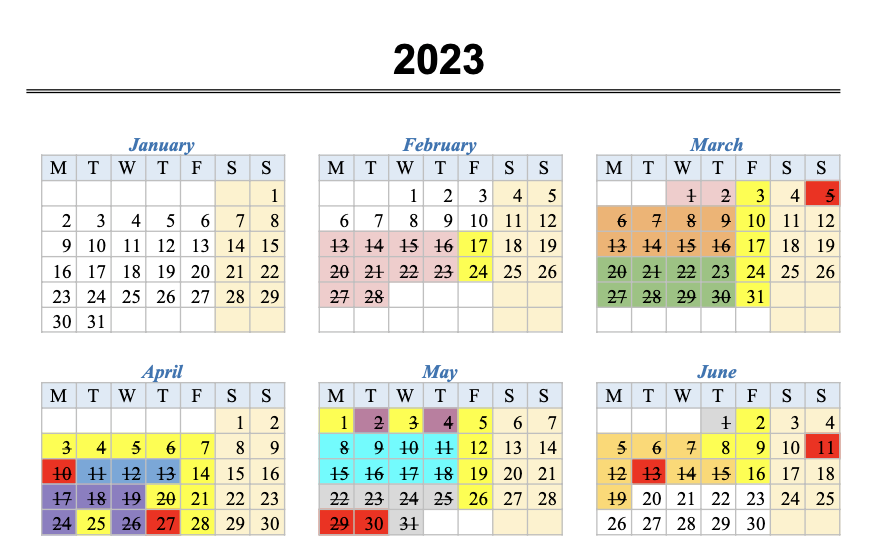
\includegraphics[width=\linewidth]{figures/cal.png}
		\caption{Calendar with Sprint Distribution and Daily Records}
		\label{fig:cal}
	\end{minipage}
	\hfill
	\begin{minipage}[b]{0.40\textwidth}
		\centering
		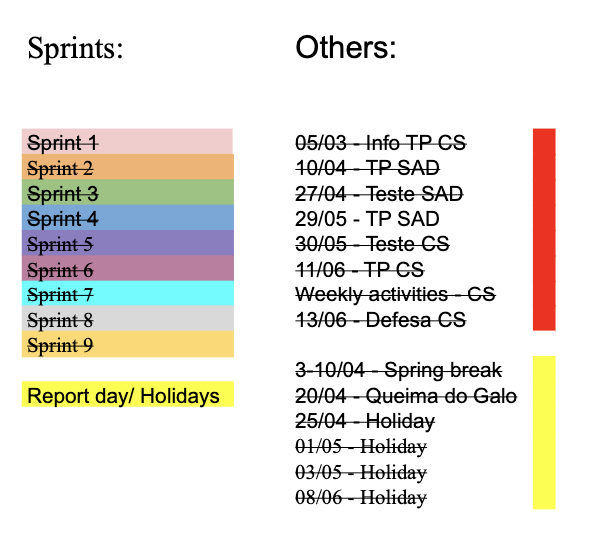
\includegraphics[width=\linewidth]{figures/leg.png}
		\caption{Calendar's caption}
		\label{fig:cap}
	\end{minipage}

\end{figure}

\noindent \rule{\linewidth}{0.4pt}
\newline
